\section{Manipulation d'un système GNU/Linux}
Dans cette partie et les parties suivantes, on considère que l'on dispose d'un système GNU/Linux avec l'interpréteur de commande Bash. Sauf mention contraire, l'ensemble des exemples et commandes devraient fonctionner sans problèmes sous toutes les distributions GNU/Linux, sous macOS et même avec le \href{https://docs.microsoft.com/fr-fr/windows/wsl/install-win10}{sous-système Linux sur Windows} (\textit{Windows sub-system for Linux}, WSL), à condition d'utiliser Bash.

\note{Note:} On parlera de \say{terminal} ou de \say{console} pour l'interface en ligne de commande (ou de \say{CLI}, pour \textit{Command Line Interface}), mais de \say{Shell} pour parler du programme sous-jacent permettant l'interprétation des commandes (Bash).

\vspace{-3mm}
\subsection{POSIX} \label{sec:POSIX}
\vspace{-3mm}
Si l'ensemble des outils GNU/Linux sont similaires sur tous les systèmes et dérivés d'UNIX, ce n'est pas un hasard. Devant la multiplication des variantes d'UNIX, \textbf{les standards POSIX (pour \textit{Portable Operating System Interface}) ont été établis en 1988} pour proposer une \textbf{interface d'utilisation commune à tous les systèmes UNIX}.

La majeure partie des commandes et des programmes présentés ci-après respectent les dernières versions de  POSIX et peuvent donc être utilisés comme indiqué sur tous les systèmes qui les proposent. \textbf{Il existe cependant quelques rares cas dans lesquels le standard n'est pas respecté} (pour des raisons philosophiques ou historiques), mais ils sont explicités au sein de leur documentation.

\subsection{Ligne de commande}

\subsubsection{Usages et intérêt}

Bien que la plupart des systèmes de bureau disposent d'une interface graphique, la gestion quotidienne du système peut se faire intégralement en ligne de commande. De nombreux programmes ne sont d'ailleurs qu'une surcouche à leur version console, pour plus de simplicité.

De manière générale, la ligne de commande permet à un utilisateur de se connecter, d'exécuter des programmes et d'interagir le système. Utiliser la ligne de commande permet également d'agir de façon plus uniforme, grâce à POSIX (voire partie \ref{sec:POSIX}).

\subsubsection{Plusieurs terminaux}
Il existe deux types de terminaux : 
\begin{itemize}
    \item Graphique (tel que \texttt{gnome-terminal}), permettant d'utiliser un terminal graphique,
    \item Terminal pur, ne permettant d'afficher que du texte.
\end{itemize}
\vspace{\baselineskip}

Il existe plusieurs terminaux, identifié par un numéro, et accessible grâce au raccourci clavier \texttt{Ctrl+Alt+<FX>}. \textbf{Par défaut, l'interface graphique s'exécute dans un terminal}, généralement le TTY7 ou le TTY1. Ainsi, le raccourci clavier \texttt{Ctrl+Alt+F2} permet de passer au TTY2 à tout moment, passant en mode terminal pur, si celui-ci existe bien.

\newpage

\subsection{Prise en main du terminal}
\vspace{-4mm}
Lorsque l'on lance un terminal, il n'y a généralement aucun affichage, seuls quelques caractères s'affichent au début de ligne. Il s'agit de l'invite de commande ou \textit{prompt}.
\subsubsection{Invite de commande -- \textit{prompt}}

Le \textit{prompt}, lorsqu'il n'est pas personnalisé\footnote{Le prompt peut-être personnalisé par la variable d'environnement (voir partie \ref{sec:env}) \texttt{PS1}. La syntaxe pouvant être complexe, des générateurs en ligne existent comme \href{http://ezprompt.net}{ESPrompt} ou \href{http://bashrcgenerator.com}{.bashrc generator}}, est généralement de la forme suivante :
\begin{nscenter}
    \texttt{login@machine:\tilde~\$}
\end{nscenter}

Si on l'analyse, peut détailler trois parties :
\begin{itemize}
    \item \texttt{login@machine}, identifie l'utilisateur courant (via son login) et la machine courante (via son nom). Cela peut paraître superflu au premier abord mais s'avère très utile lorsque l'on se connecte à plusieurs machines à distance (voir partie \ref{cmd:ssh}).
    \item \texttt{\tilde}, correspond au dossier courant. En l'occurrence, il s'agit d'un alias qui correspond au dossier personnel de l'utilisateur courant (voir partie \ref{sec:dirhome}). En changeant de dossier, cette valeur changera pour le nom ou le chemin du nouveau dossier.
    \item \texttt{\$}, correspond au niveau d'utilisateur. \texttt{\$} signifie utilisateur normal, \texttt{\#} signifie super-utilisateur. L'utilisateur normal peut, le temps d'une commande, acquérir les droits de super-utilisateur (voir partie \ref{cmd:sudo}), sans que ce symbole change.
\end{itemize}\vspace{1mm}

Lorsque le \textit{prompt} est affiché, cela signifie que l'on peut entrer une commande.

\subsubsection{Structure d'une commande} \label{sec:command}

Une commande, quel que soit le système d'exploitation, est une chaîne de caractère que l'on va taper au clavier pour réaliser une action sur le système. Elle se compose de plusieurs mots ou codes, \textbf{les arguments}, séparés par au moins un espace. On représente une commande ainsi :
\begin{nscenter}
    \mintinline{bash}{command [ --long-option | -o -p <value> -t ] parameter}
\end{nscenter}
\begin{itemize}
    \item \texttt{command} - La commande est presque toujours en minuscule, parfois composés de plusieurs mots, séparés par des tirets (\texttt{-}) ou des sous-tirets (\texttt{\_}) ;
    \item Les arguments entre crochets (\texttt{[]}) sont facultatifs, ce sont des options ;
    \item les arguments séparés par des \textit{pipes} (\texttt{|}) indiquent une alternative : ils sont exclusifs et ne peuvent être utilisés simultanément ;
    \item les argument entre chevrons (\texttt{<>}) sont à remplacer par le texte voulu. Ils ne sont pas toujours entre chevrons mais différencié des autres arguments (majuscules, couleurs\dots)
\end{itemize}
\note{Note :} On présente souvent une commande ou une séries de commandes, en précédant la ou les lignes par le symbole de niveau d'utilisateur, qui ne fait alors pas partie de la commande.

\paragraph{Notation des arguments d'options}

Il existe deux types d'arguments d'options : les arguments courts et les arguments longs.
\begin{itemize}
    \item Les arguments courts commencent par un tiret et ne comportent qu'une seule lettre (voir chiffre, dans de très rares cas), majuscule ou minuscule.  Ils peuvent nécessiter une valeur, qui est alors précisée par le paramètre suivant : \mintinline{bash}{command -o -p -t value}.\newline
    Il est possible de combiner les paramètres courts pour plus de simplicité : \mintinline{bash}{command -opt}\vspace{\baselineskip}
    
    \item Les arguments longs commencent par un double tiret et comportent généralement un mot complet ou plusieurs mots séparés par des tirets (\texttt{-}) ou des sous-tirets (\texttt{\_}). Leur valeur peut aussi être donnée via un signe égal (\texttt{=}): \mintinline{bash}{command --option value --long-option=true}
\end{itemize}
\newpage

Les arguments de chaque commande sont explicités dans le manuel. Pour consulter le manuel d'une commande, il suffira d'utiliser la commande \texttt{\cmdref{man} <command>} (voir partie \ref{cmd:man}).

\warning{Enfin, une commande dispose toujours (même s'ils ne sont pas utilisés):}
\begin{itemize}
    \item D'un code de retour (ou code d'erreur) (voir partie \ref{sec:error}),
    \item D'une entrée sur laquelle elle peut lire des données (voir partie \ref{sec:redirect}),
    \item D'une sortie sur laquelle elle peut écrire des données (voir partie \ref{sec:redirect}),
    \item D'une sortie d'erreur, dédiée au messages d'erreur (voir partie \ref{sec:redirect}).
\end{itemize}

\subsubsection{Premières commandes}

Les premières commandes essentielles à apprendre permettent d'obtenir des informations sur la sessions courante ou le système. Elles sont détaillées dans le tableau \ref{tab:first_cmd}.
\begin{table}[bh!]
    \centering
    \begin{tabularx}{\textwidth}{| c | X |}  \hline
        \textbf{Commande} & \textbf{Description}                                                                                                \\ \hline
        \texttt{whoami} \command{whoami}  & Affiche le login de l'utilisateur courant.                                                          \\ \hline
        \texttt{pwd} \command{pwd}        & Affiche le dossier courant (\textit{PoWer Directory}). Plus de détails partie \ref{sec:directories}.\\ \hline
        \texttt{echo} \command{echo}      & Affiche le message passé en premier paramètre. Avec \texttt{-n}, pas de saut de ligne.              \\ \hline
        \texttt{apropos} \command{apropos}& Recherche les commandes relatives au mot-clé passé en premier paramètre.                            \\ \hline
        \texttt{history} \command{history}& Affiche les commandes récentes (le nombre est passé en paramètre).                                  \\ \hline
        \cmdref{man}                      & Affiche le manuel d'utilisation de la commande passée en paramètre.                                 \\ \hline
        \texttt{info} \command{info}      & Alternative à \cmdref{man} proposée par GNU, basée sur des sections navigables.                        \\ \hline
        \texttt{help} \command{help}      & Affiche l'aide pour les commandes internes de Bash sans page de manuel.                             \\ \hline
    \end{tabularx}
    \caption{Commandes basiques permettant d'obtenir des informations sur le système.}
    \label{tab:first_cmd}
\end{table}
\vspace{-4mm}

Hormis quelques rares exceptions, les commandes sont toutes des programmes. Cela signifie qu'un exécutable est présent sur le système et est appelé lorsque l'on valide la commande. Ce fonctionnement est possible grâce à la variable d'environnement \texttt{\$PATH}, détaillée partie \ref{sec:env}.

\subsubsection{À propos du manuel -- \texttt{man}} \command{man}

Le manuel regroupe la documentation de toutes les commandes installées sur le système. Il existe plusieurs sections de manuel, allant de 1 à 9. Ces sections sont décrites dans le manuel de la commande \cmdref{man}, consultable grâce à la commande \mintinline{bash}{man man}. On notera que la section \texttt{1} contient les pages de manuel des commandes Bash. Dans le cas ou une page de manuel a des homonymes dans d'autres sections, on peut forcer la section \texttt{X} : \mintinline{bash}{man X command}

La plupart des pages de manuel comportent une présentation succincte de la commande (le synopsis) ainsi qu'une description de la commande, de ses cas d'usages et de ses paramètres. Il y a généralement une partie définissant les codes de retour possibles et leur signification. Certaines pages on également des exemples d'utilisations et de résultats attendus.

En général, lorsqu'on utilise le manuel, on dispose d'une interface dédiée. On peut naviguer dans le manuel avec les flèches directionnelles et les touches \texttt{PageUp} et \texttt{PageDown}. Pour effectuer une recherche, on tapera un \textit{slash} (\texttt{/}) suivi du mot clé à rechercher, puis \texttt{Entrée}. \texttt{N} passera à la prochaine occurrence et \texttt{P} à l'occurrence précédente. \texttt{Q} permet de quitter.

Il se peut cependant que certaines commandes ne bénéficient pas de page de manuel ni d'aide. Dans ce cas, on peut essayer d'appeler la commande avec l'option \texttt{--help} ou \texttt{-h}. Cette option affiche généralement comment utiliser la commande et les arguments qu'elle peut prendre.

\newpage

\vspace{-4mm}
\subsubsection{Raccourcis de saisie}
\vspace{-2mm}

Le terminal étant conçu pour être utilisé intégralement au clavier, il existe de nombreux raccourci pour faciliter la saisie et le déplacement du curseur. Des éléments plus précis sur la notation des raccourcis clavier figurent en annexe \ref{appendix:shortcuts}.

\begin{table}[h!]
    \centering
    \begin{tabularx}{\textwidth}{| c | X |}  \hline
        \textbf{Raccourci} & \textbf{Effet} \\ \hline
        \texttt{Tab}      & Auto-complète le nom de commande courant ou le chemin si possible. \newline                                                                                                  Appuyer deux fois de suite pour voir la liste des suggestions. \\  \hline
        \texttt{\textuparrow} \scriptsize{(flèche haut)}    & Affiche la commande précédente dans l'historique. \\  \hline
        \texttt{\textdownarrow} \scriptsize{(flèche bas)}   & Affiche la commande suivante dans l'historique. \\  \hline
        \texttt{Ctrl + L} & Nettoie l'écran de tout affichage. Sous macOS, nettoie jusqu'à la commande précédente. \\  \hline
        \texttt{Ctrl + C}                                   & Interrompt l'exécution de la commande en cours. \\  \hline
        \texttt{Ctrl + Z} & Mets la commande en cours d'exécution en pause, pour la reprendre plus tard. \newline                                                                                                       Voir partie \ref{sec:tasks}. \\  \hline
        \texttt{Ctrl + D} & Interrompt la saisie lorsqu'une commande en attend une.  \newline                                                                                                                           Permet aussi de quitter le Shell. \\  \hline
        \texttt{Ctrl + \textleftarrow}                      & Déplace le curseur au mot précédent. Équivalent à \texttt{Alt+B}. \\  \hline
        \texttt{Ctrl + \textrightarrow}                     & Déplace le curseur au mot suivant. Équivalent à \texttt{Alt+F}.\\  \hline
        \texttt{Ctrl + R} & Recherche dans l'historique des commandes en tapant quelques caractères. \newline
                            Retaper le raccourci pour passer à la commande correspondante précédente. \\  \hline
        \texttt{Ctrl + S}                                   & Pause le défilement d'affichage de la commande en cours d'exécution. \\  \hline
        \texttt{Ctrl + Q}                                   & Reprend l'exécution de la commande mise en pause par \texttt{Ctrl + S}. \\  \hline
    \end{tabularx}
    \caption{Principaux raccourcis clavier dans un terminal Linux}
    \label{tab:kbd_shortcuts}
\end{table}

De plus, les flèches de déplacement traditionnelles sont bien évidemment utilisables. On notera tout de même les touches suivantes : 
\begin{itemize}
    \item \texttt{Home} ou \texttt{Début} ou \texttt{$\nwarrow$}, qui permet de revenir au début de la commande ou de la ligne.
    \item \texttt{End} ou \texttt{Fin}, qui permet d'aller à la fin de la commande ou de la ligne.
\end{itemize}

\medskip

Enfin, la souris peut être utile si l'on dispose d'un environnement graphique : 
\begin{table}[h!]
    \centering
    \begin{tabularx}{\textwidth}{| c | X |}  \hline
        \textbf{Raccourci souris}   &   \textbf{Effet} \\ \hline
        \texttt{Clic gauche}        &   Sélectionne le texte et le copie. \\  \hline
        \texttt{Clic droit}         &   Colle le texte copié \warning{OU} affiche le menu contextuel. \\  \hline
        \texttt{Clic molette}       &   Colle le texte copié. \\  \hline
    \end{tabularx}
    \caption{Principaux raccourcis souris dans un terminal Linux graphique}
    \label{tab:mouse_shortcuts}
\end{table}
\vspace{-7mm}

\note{Note :} Ces raccourcis peuvent varier légèrement en fonction du système ou de l'interface utilisée. Les raccourcis de déplacement du curseur sont généralement utilisables au sein de l'ensemble des éditeurs de texte.

\paragraph{Rappeler la dernière commande}
Il est possible d'utiliser deux points d'exclamation (\texttt{!!}) pour réutiliser la dernière commande. On peut la compléter et la combiner avec n'importe quelle autre commande. Ce raccourci est notamment utilisé pour rappeler la dernière commande avec les droits du super-utilisateur : \texttt{sudo !!} (voir partie \ref{sec:su}).

\newpage
\subsection{Système de fichier}
\vspace{-2mm}
%Plusieurs commandes sont disponibles pour pouvoir afficher, se déplacer et manipuler l'arborescence de fichiers détaillée dans la partie \ref{sec:directories}).

\subsubsection{Commandes de manipulation}

\paragraph{\texttt{ls}} \command{ls}
\textbf{L}i\textbf{s}te un dossier dont le chemin le chemin (absolu ou relatif) est passé en paramètre. Sans paramètre, elle affichera le contenu du dossier courant. Lorsque le chemin donné est celui d'un fichier qui n'est pas un dossier, il est listé seul. \newline
\cmdref{ls} dispose de plusieurs options : 
\begin{itemize}
    \item \texttt{-a} : Affiche tous les fichiers, y compris les fichiers cachés. 
    \item \texttt{-H} : En combinaison avec \texttt{-l}, affiche la taille des fichiers en multiples de 1024 octets plutôt qu'en octets. On parle de taille lisible par l'\textbf{h}umain.
    \item \texttt{-l} : Affiche les informations détaillées.
    Dans ce mode, plusieurs informations sont détaillées, avec uniquement un fichier par ligne. Chaque élément de ligne contient différentes informations (voir figure \ref{fig:lsl}). Le type est détaillé dans la partie \ref{sec:filetypes}, les droits d'usages sont détaillés dans la partie dédiée à \cmdref{chmod}, la notion de propriétaires est détaillée dans la partie \ref{sec:users}.
\end{itemize}

\begin{figure}[h!]
        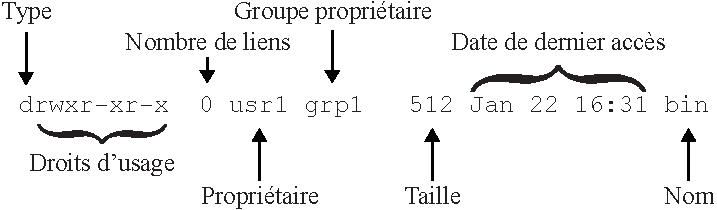
\includegraphics{res/lsl.pdf}
        \centering
        \caption{Détail de l'affichage détaillé de \texttt{ls}.}
    \label{fig:lsl}
\end{figure}

\paragraph{\texttt{cd}} \command{cd}
Permet de se déplacer vers le dossier dont le chemin (absolu ou relatif) est passé en paramètre. Si aucun paramètre n'est donné, retourne au dossier personnel (\texttt{\tilde}).
\begin{itemize}
    \item \texttt{-} : Retourne au dossier précédent. Un second appel à \mintinline{bash}{cd -} retourne au premier dossier car il n'y a pas d'historique.
\end{itemize}
\vspace{3mm}

\note{Note :} Les commandes \texttt{pushd}\command{pushd} et \texttt{popd}\command{popd} permettent de gérer un historique des dossiers sous forme de pile, permettant ainsi de faciliter le retour aux dossiers précédents. \newline 
De plus, le programme \texttt{ranger}\command{ranger} (non installé par défaut) permet un affichage et une navigation plus visuelle, mais ne peut pas être utilisé dans un script.

\paragraph{\texttt{mkdir}} \command{mkdir}
Créé les dossiers passés en paramètres. Il peut s'agir de chemins complets (relatifs ou absolus) ou juste de noms de dossiers à créer.
\begin{itemize}
    \item \texttt{-p} : Créé tous les dossiers parents nécessaires et ne renvoie pas d'erreur si le dossier existe.
    \item \texttt{-m <perm>} : Créé le dossier avec les droits d'accès donnés, à la manière de \cmdref{chmod} (voir partie \ref{sec:chmod}).
\end{itemize}

\paragraph{\texttt{rm}} \command{rm}
Supprime les fichiers ou dossiers passés en paramètres.
\begin{itemize}
    \item \texttt{-i} : Mode interactif. Demande confirmation avant suppression de chaque éléments.
    \item \texttt{-f} : Mode forcé. Suppression du fichier sans confirmation.
    \item \texttt{-r} : Mode récursif. Supprime récursivement un dossier et tous ses sous-dossiers.
\end{itemize}
\vspace{3mm}

\note{Note :} La commande \texttt{rmdir}\command{rmdir} permet de supprimer un ou plusieurs dossiers vides.

\newpage

\paragraph{\texttt{cp}} \command{cp}
Copie les fichiers ou dossiers passés en paramètres vers le dernier paramètre. Si plusieurs fichiers sont à copiés, le dernier paramètre doit être un dossier.
\begin{itemize}
    \item \texttt{-i} : Mode interactif. Demande confirmation avant d'écraser le fichier de destination (s'il existe).
    \item \texttt{-f} : Mode forcé. Écrasement du fichier de destination (s'il existe) sans confirmation.
    \item \texttt{-r} : Mode récursif. Copie récursivement le contenu d'un dossier.
    \item \texttt{-u} : Mode mise-à-jour (\textit{\textbf{U}pdate}). Ne copie les fichiers vers la destination que si la source est plus récente ou que la destination n'existe pas.
\end{itemize}

\paragraph{\texttt{mv}} \command{mv}
Déplace ou renomme les fichiers ou dossiers passés en paramètres. Utilisation similaire à \cmdref{cp}.
\begin{itemize}
    \item \texttt{-i} : Mode interactif. Confirmation préalable avant écrasement du fichier de destination, s'il existe.
    \item \texttt{-f} : Mode forcé. Écrasement du fichier de destination (s'il existe) sans confirmation.
    \item \texttt{-u} : Mode mise-à-jour (\textit{\textbf{U}pdate}). Ne copie les fichiers vers la destination que si la source est plus récente ou que la destination n'existe pas.
\end{itemize}

\paragraph{\texttt{touch}} \command{touch}
Modifie la date de dernier accès d'un fichier ou le créé s'il n'existe pas.

Toutes les commandes précédentes peuvent traiter un ou plusieurs fichiers ou dossiers. De plus, si le paramètre comprend un astérisque (\texttt{*}), alors Bash fera correspondre les noms de fichiers au mieux. Ainsi si on effectue \mintinline{bash}{rm i*}, Bash supprimera l'ensemble des fichiers ou dossiers dans le dossier courant qui commencent par \texttt{i}.

\paragraph{\texttt{cat}} \command{cat}
Affiche le contenu d'un fichier directement dans le terminal.
\begin{itemize}
    \item \texttt{-} : Si aucun fichier n'est passé en paramètre, attends une entrée au clavier, puis l'affiche à chaque entrée. Utiliser \texttt{Ctrl+D} pour terminer la saisie. Utile au sein de boucles \cmdref{while}.
    \item \texttt{-n} : Préfixe chaque ligne du fichier par le numéro de ligne
\end{itemize}

\paragraph{\texttt{less} -- \texttt{more} -- \texttt{most}} \command{less}\command{more}\command{most}
Ces trois commandes sont des afficheurs de texte. Contrairement à \cmdref{cat}, ils permettent à l'utilisateur de faire défiler le fichier. Pour sortir de l'afficheur, il suffit d'appuyer sur \texttt{Q}.

\begin{itemize}
    \item \texttt{less} : Permet de remonter ou de descendre la lecture du fichier.
    \item \texttt{more} : Ne permet que de descendre dans la lecture du fichier.
    \texttt{Entrée} descend d'une ligne, \texttt{Espace} passe à la \say{page} suivante).
    \item \texttt{most} : Identique à \cmdref{less}, mais gère également les couleurs lorsque possible.
\end{itemize}\vspace{-3mm}

\note{Note :} C'est en général un de ces afficheurs qui est utilisé pour consulter le \cmdref{man}. Ce comportement est modifiable via la variable d'environnement \texttt{\$PAGER} (voir partie \ref{sec:env}).

\paragraph{\texttt{nano} -- \texttt{vim} -- \texttt{emacs}}
Il existe également des éditeurs de texte, pouvant lire et écrire des fichiers depuis la ligne de commande, les plus connus étant \cmdref{nano}, \cmdref{vim} et \cmdref{emacs}. Leur utilisation étant très spécifiques, leur fonctionnement est détaillé dans les annexes dédiées (\ref{appendix:nano}, \ref{appendix:vim} et \ref{appendix:emacs}). \newline
Ces éditeurs peuvent être utilisés directement par d'autres commandes (telles que \texttt{git}) grâce à la variable d'environnement \texttt{\$EDITOR} (voir partie \ref{sec:env}).

\paragraph{\texttt{ne}}\command{ne}
\cmdref{ne} (pour \textit{\textbf{N}ice \textbf{E}ditor}) texte se différencie des précédents par l'utilisation des raccourcis claviers usuels et dispose d'un menu déroulant que l'on peut afficher avec \texttt{F1}.

\newpage
\subsubsection{Types de fichiers} \label{sec:filetypes}

Comme vu dans la figure \ref{fig:lsl}, il existe différents types de fichiers sous Linux.

\paragraph{Fichiers simples}
Il s'agit du type de fichier le plus naturel. Un fichier simple contient des données écrites sur le disque, qui peuvent être lues directement.
Il existe deux types de fichiers simples : les fichiers textes et les fichiers binaires.

Les fichiers textes sont composés de chaînes de caractères, écrites lignes par lignes. Il peuvent être lus dans n'importe quel afficheur ou éditeur de texte. Il faut noter que les lignes sont séparés par un caractère spécial, invisible par défaut, que l'on appelle saut de ligne (\textit{Line Feed} en anglais, abrégé en \textit{LF}). On le voit très régulièrement sous la notation \texttt{\textbackslash n}. Sous Windows, les sauts de lignes sont marqués en plus par un retour à la ligne (\textit{Carriage Return}) : abrégés en \textit{CR-LF}, notés \texttt{\textbackslash r\textbackslash n}. C'est pourquoi les fichiers Linux sont souvent mal affiché sous Windows.

Il existe plusieurs encodages du texte. Le plus ancien est le code ASCII, qui définit un encodage des caractères sur 8 bits dans sa version étendue, mais ne permet donc d'encoder que 255 caractères. La plupart des encodages dédiés à notre alphabet tentent de respecter le code ASCII, pour des raisons historiques de compatibilité. On rencontre également l'encodage UTF-8 (pour \textit{\textbf{U}niversal coded character set \textbf{T}ransformation \textbf{F}ormat - 8 bits}). UTF (ou Unicode) permet de coder la quasi totalité des caractères utilisés dans le monde, y compris les emojis.

Les fichiers binaires, quant à eux, sont stockés purement sous forme binaire et n'ont pas vocation à être lus comme un fichier texte. Ils peuvent contenir toute sorte d'information. Il s'agit souvent de code compilé, prévu pour être exécuté (des programmes ou bibliothèques), de données de média (image, vidéos, sons\dots), ou d'autres données, gérées par des programmes spécifiques (archives, données de jeux\dots).

\textbf{Le caractère des fichiers simples dans l'affichage détaillé de \cmdref{ls} est un tiret (\texttt{-})}.

\paragraph{Dossiers}
Comme évoqué précédemment, les dossiers sous considérés comme des fichiers particuliers sous Linux. Il est à noter qu'un dossier donné occupe un espace en lui-même sur le disque dur, sans parler de la taille totale des fichiers qu'il contient. En effet, l'information du dossier (emplacement, droits d'utilisation et nom) doit être stocké. Cette taille est cependant très réduite et commune à l'ensemble des dossiers. Dans la figure \ref{fig:lsl}, elle vaut 512 octets, ce qui correspond à la taille minimale d'allocation d'espace sur le disque dur.\newline 
\textbf{Le caractère des dossiers dans l'affichage détaillé de \cmdref{ls} est \texttt{d}}.

\paragraph{Liens symboliques} \label{sec:file_links}
Les liens symboliques sont des fichiers qui ne contiennent qu'une référence (un pointeur) vers un autre fichier. Cela permet d'utiliser le lien symbolique comme s'il s'agissait du fichier et ainsi d'avoir plusieurs noms ou chemin pour représenter le même fichier sans le dupliquer. Les liens symboliques sont notamment utilisés pour pouvoir changer de version entre différents programmes ou fichier facilement. De nombreuses commandes permettent de définir si l'on souhaite agir sur le lien en lui même ou sur le fichier qu'il pointe. Si le fichier pointé par le lien n'existe pas, on dit que le lien est cassé, rompu, ou orphelin. \newline
\textbf{Le caractère des liens symboliques dans l'affichage détaillé de \cmdref{ls} est \texttt{l}}.

\vspace{5mm}
\begin{nscenter}
\textbf{Ces types de fichiers sont les principaux à retenir.} \\
Les types suivants sont bien moins courants et la compréhension de leur fonctionnement relève d'un usage avancé des systèmes Linux et de Bash.
\end{nscenter}

\newpage

\paragraph{\textit{Sockets}} \label{sec:file_sockets}
Les \textit{sockets} sont des fichiers particuliers utilisés pour échanger des données entre les programmes. Une \textit{socket} ne stocke donc les données que jusqu'à ce qu'elles soient lues, paquets par paquets. C'est également un mécanisme utilisé pour la communication réseau. \newline \textbf{Le caractère des \textit{sockets} dans l'affichage détaillé de \cmdref{ls} est \texttt{s}}.

\paragraph{\textit{Pipes}} \label{sec:file_pipes}
Les \textit{pipes} (ou tubes) ont un fonctionnement similaire aux \textit{sockets}, mais agissent par flux et non pas par paquets. La lecture dans un \textit{pipe} se fait caractère par caractère. Ils permettent d'agir comme un lien entre un producteur (celui qui va écrire dans le \textit{pipe}) et un consommateur (le lecteur). L'usage des \textit{pipes} en Bash est courant. Il repose sur le même concept, avec une implémentation technique légèrement différente. Son usage est détaillé en partie \ref{sec:pipes}. \newline
\textbf{Le caractère des \textit{pipes} dans l'affichage détaillé de \cmdref{ls} est \texttt{p}.}

\paragraph{Blocs d'appareils} \label{sec:file_dev}
Les fichiers de blocs d'appareils (\textit{Block devices} en anglais) sont une représentation d'un périphérique, tels qu'un disque dur. On les trouve notamment dans le dossier \texttt{/dev} (voir partie \ref{sec:dirdev}). Il s'agit d'une sorte d'interface d'interaction bas niveau avec les périphériques. \newline
\textbf{Le caractère des \textit{block devices} dans l'affichage détaillé de \cmdref{ls} est \texttt{d}.}

\paragraph{\textit{Character device}} \label{sec:file_char}
Les fichiers de \textit{character devices} permettent une lecture ou écriture d'un flux de données. Ils sont notamment utilisés pour représenter des appareils comme une carte son. D'autres exemples notables de ce type de fichiers sont :
\begin{itemize}
    \item \texttt{/dev/zero}, qui ne laisse lire que des zéros,
    \item \texttt{/dev/null}, qui peut lire n'importe quel caractère sans rien stocker,
    \item \texttt{/dev/random} qui retourne des données aléatoires.
\end{itemize}
Les terminaux TTY sont également des fichiers de type \textit{character devices}. \newline
\textbf{Le caractère des \textit{char devices} dans l'affichage détaillé de \cmdref{ls} est \texttt{c}.}

On a vu que pour obtenir des informations sur un fichier, sans le lire, on peut utiliser \mintinline{bash}{ls -l}. D'autres informations peuvent être obtenues, sur le type de fichier et son contenu grâce à la commande \cmdref{file}.

\paragraph{\texttt{file}} \command{file}
Affiche les informations sur les fichiers donnés en paramètre : le type de fichier s'il ne s'agit pas d'un fichier simple, et des informations sur le contenu du fichier (image, document, texte...) sinon.
\begin{itemize}
    \item \texttt{-i} : Pour les fichiers simples, affiche le type de fichier sous la forme standardisée MIME.
    \item \texttt{-L} : Pour les liens symboliques, affiche les information sur le fichier cible plutôt que sur le lien lui-même.
\end{itemize}

\newpage

\subsection{Utilisateurs, groupes et droits d'accès} \label{sec:users}
\vspace{-2mm}
GNU/Linux est un système multi-utilisateurs. Ainsi, plusieurs utilisateurs peuvent utiliser le système simultanément. Chaque utilisateur a un identifiant unique : \textit{UID}. Il existe également des groupes, pouvant réunir un ou plusieurs utilisateurs. Chaque utilisateur est automatiquement membre d'un groupe du même nom : son groupe principal. De plus, il existe généralement des groupes dédiés à des programmes ou services particuliers. De même que pour les utilisateurs, un groupe possède un identifiant unique : le \textit{GID}. Les informations d'identifiants et de groupes sont consultable avec la commande \cmdref{id}.

\paragraph{\texttt{id}} \command{id}
Affiche les identifiants de l'utilisateur passé en paramètre, ou de l'utilisateur courant sinon.
\begin{itemize}
    \item \texttt{-G} : Affiche tous les GID de l'utilisateur.
    \item \texttt{-u} : Affiche l'UID de l'utilisateur.
    \item \texttt{-n} (en combinaison avec \texttt{-G} ou \texttt{-u }) : affiche le nom de l'item demandé, pas l'ID.
\end{itemize}\vspace{\baselineskip}

La liste des utilisateurs figure dans le fichier \texttt{/etc/passwd}. Ce fichier contient, pour chaque utilisateur (un par ligne), les informations essentielles (comme le nom, le mot de passe, le dossier personnel...) séparées par des deux-points (\texttt{:}). De la même manière, les groupes utilisateurs sont détaillés dans le fichier \texttt{/etc/group}.

Les notions d'utilisateurs et de groupes permettent d'attribuer des droits d'accès spécifiques pour chaque fichier du système. Les droits accès d'utilisateurs peuvent être restreints pour plus de sécurité et éviter à un utilisateur d'accéder aux données d'un autre ou, au contraire, étendus pour permettre le partage de données. Ainsi, certaines actions ou programmes systèmes peuvent nécessiter d'avoir des droits spécifiques pour être effectuées ou utilisés.

\subsubsection{Droits d'accès - \texttt{chmod}} \label{sec:chmod}
\vspace{-3mm}

Sous les systèmes UNIX, la gestion des droits utilisateurs est rendue possible grâce aux notions de droits d'accès et de groupes. Chaque utilisateur appartient à un groupe ou plusieurs groupes d'utilisateurs. Chaque utilisateur et chaque groupe dispose de droits d'accès spécifiques. On parle également de mode de fichier, car chaque fichier possède un unique propriétaire et un unique groupe propriétaire.

Il existe trois niveaux de droits d'accès pour tous les fichiers : 
\begin{enumerate}
    \item Utilisateur (\textit{\textbf{U}ser}): ce sont les droits de l'utilisateur courant,
    \item Groupe (\textit{\textbf{G}roup}): ce sont les droits du groupe auquel l'utilisateur courant appartient,
    \item Autres (\textit{\textbf{O}thers}) : ce sont les droits de tous les utilisateurs des autres groupes.
\end{enumerate}
On fait généralement référence à ces niveaux par leur initiale. Si l'on fait référence à tous les utilisateurs, on utilisera la lettre \texttt{a} (\textit{\textbf{A}ll}).

Pour chacun de ces trois niveaux, il existe trois types d'accès :
\begin{enumerate}
    \item Lecture (\textit{\textbf{R}ead}) : le droit de lire le fichier ou le contenu du dossier,
    \item Écriture (\textit{\textbf{W}rite}) : le droit de créer ou modifier le fichier ou dossier,
    \item Exécution (\textit{\textbf{E}xecute}) : le droit d'ouvrir le dossier ou d'exécuter le fichier.
\end{enumerate}

\newpage

Ceci peut se représenter sous forme d'un triplet Lecture-Écriture-Exécution pour chacun des trois niveaux de droits d'accès. Il existe plusieurs représentations possibles de ce triplet, comme détaillé dans le tableau \ref{fig:chmod} : textuelle, binaire ou octale.

\begin{table}[h!]
    \begin{tabular}{|c|c|c|l|}
        \hline
        \textbf{Utilisateur (\texttt{u})}   &   \textbf{Groupe} (\texttt{g})&   \textbf{Autres} (\texttt{o})&   \textbf{Représentation}                 \\ \hline
        \texttt{r-{}-}                        &   \texttt{-w-}                &   \texttt{--x}                &   Textuelle (\texttt{\cmdref{ls} -l})     \\ \hline
        \texttt{100}                        &   \texttt{010}                &   \texttt{001}                &   Binaire                                 \\ \hline
        \texttt{4}                          &   \texttt{2}                  &   \texttt{1}                  &   Octale                                  \\ \hline
    \end{tabular}
    \centering
    \caption{Détail des représentations possibles des trois triplets de droit d'accès}
    \label{fig:chmod}
\end{table}

Pour chaque niveau d'accès, si on additionne la valeur numérique des types d'accès autorisés, on obtient un triplet d'entiers compris entre 0 et 7. On représente souvent les droits d'accès sous cette forme, dite octale, car elle est plus concise, comme l'illustrent les exemples du tableau \ref{fig:chmod_example}


\begin{table}[h!]
    \begin{tabularx}{\textwidth}{|X|c|c|c|c|}
    \hline
\multicolumn{1}{|c|}{\multirow{2}{*}{\textbf{Droits d'accès et description}}}                                     & \multicolumn{2}{|c|}{\textbf{Propriétaire}} & \multicolumn{2}{|c|}{\textbf{Représentation}} \\
                                                                                                                & \textbf{Utilisateur} & \textbf{Groupe}    & \textbf{Textuelle} & \textbf{Octale}        \\ \hline
Lecture et exécution pour tous, modifiable par son propriétaire (par exemple, script partagé sans modification) & \texttt{user1}       & \texttt{user1}     & \texttt{rwxr-xr-x} & \texttt{755}           \\ \hline
Fichier de notes partagées au sein du groupe                                                                    & \texttt{user1}       & \texttt{users}     & \texttt{rw-rw-{}-{}-{}-} & \texttt{660}           \\ \hline
Fichier confidentiel (non éditable, lisible par son propriétaire)                                               & \texttt{user1}       & \texttt{user1}     & \texttt{r-{}-{}-{}-{}-{}-{}-{}-} & \texttt{400}           \\ \hline
Dossier partagé (contenu visible et \texttt{cd} dans le dossier possible par tous)                              & \texttt{user2}       & \texttt{users}     & \texttt{rwxr-xr-x} & \texttt{755}           \\ \hline            
\end{tabularx}
    \centering
    \caption{Exemples de représentations des droits d'accès}
    \label{fig:chmod_example}
\end{table}

\paragraph{\texttt{chmod}} \command{chmod}
Permet de \textbf{ch}anger le \textbf{mod}e d'un fichier, c'est à dire ces droits d'accès. Il prend en paramètre les changements de mode à effectuer et les fichiers ou dossiers à modifier. Le mode peut être donné sous forme octale ou textuelle.
\begin{itemize}
    \item \texttt{-R} : Mode récursif. Applique le changement récursivement à tous les fichiers et dossiers contenu dans un dossier.
\end{itemize}\vspace{\baselineskip}

Sous forme octale, il suffit de spécifier les trois chiffres : \mintinline{bash}{chmod 644 file}
 
Sous forme textuelle : il faut préciser le(s) niveau(x) d'accès concerné(s) (\texttt{u}, \texttt{g}, \texttt{o} ou \texttt{a}), l'opération à effectuer (\texttt{+}, \texttt{-} ou \texttt{=}), et les type d'accès concernés (\texttt{r}, \texttt{w}, \texttt{x}). Ainsi, pour ajouter les droits d'exécution sur le fichier \texttt{script.sh} pour l'utilisateur courant, on utilisera : \mintinline{bash}{chmod u+x script.sh}

Il est également possible de cumuler les opérateurs. Pour ajouter les droits d'écriture à l'utilisateur et au groupe tout en leur enlevant les droits d'exécution, on utilisera : \mintinline{bash}{chmod ug+w-x file}

De plus, en cas de besoin, on peut également enchaîner changements : \mintinline{bash}{chmod ug+w-x,o+r file}

\note{Note :} Bien évidemment, il faut être propriétaire du fichier (ou super-utilisateur, voir partie \ref{sec:su}) pour pouvoir modifier ses droits d'accès.

\newpage
\subsubsection{Changer d'utilisateur et droits d'administrations - \texttt{su} et \texttt{sudo}} \label{sec:su}

\paragraph{\texttt{sudo}} \command{sudo}

Sous les systèmes UNIX, il existe toujours un utilisateur spécial : le super-utilisateur ou administrateur ou \texttt{root}), dont l'UID est toujours \texttt{0}. Cet utilisateur peut modifier tous les fichiers et exécuter tous les programmes, indépendamment des droits d'accès. Il est donc particulièrement puissant. C'est la raison pour laquelle ce compte est parfois désactivé pour éviter la connexion en tant que \texttt{root}. Pour effectuer les opérations importante, il faudra que le compte utilisateur aie le droit d'obtenir les droits du super-utilisateur temporairement. C'est à cela que sert la commande \cmdref{sudo}.
\vspace{1em}

\begin{boxed}
\begin{nscenter}
\vspace{-1em}\warning{La commande \cmdref{sudo} doit uniquement être utilisée lorsque l'opération voulue nécessite les droits d'administrateur ! \newline Ce n'est pas nécessaire une solution à un message d'erreur, même si le résultat apparaît être celui recherché ! \newline Il faut toujours penser à deux fois avant de passer en mode super-utilisateur !}%
\end{nscenter}
\end{boxed}

La raison des limitations et mises en garde autour du super-utilisateur est simple : elles permettent de sécuriser le système en empêchant les virus, mauvaises manipulations ou individus malveillants d'endommager le système. Il est en effet bien plus difficile d'endommager un système en tant qu'utilisateur standard.

\paragraph{\texttt{su}} \command{su}
\textit{\textbf{S}ubstitute \textbf{U}ser}: permet de devenir temporairement l'utilisateur passé en paramètre. Sans nom d'utilisateur mentionné, il s'agira de \texttt{root}. Le mot de passe sera demandé si nécessaire.
\begin{itemize}
    \item \texttt{-l} ou \texttt{-} : Le paramètre suivant mentionne le nom d'utilisateur.
    \item \texttt{-c} : les paramètres suivants mentionnent la commande à exécuter.
\end{itemize}\vspace{\baselineskip}


\subsubsection{Propriétaire d'un fichier - \texttt{chown}}

Comme évoqué dans la partie précédente, chaque fichier possède un unique propriétaire et un unique groupe propriétaire.

Seul le super-utilisateur peut changer le propriétaire d'un fichier.

\paragraph{\texttt{chown}}  \command{chown}
Permet de changer le propriétaire de fichiers ou dossiers. Prends au moins deux paramètres : le nouveau propriétaire et les fichiers concernés.
Le nouveau propriétaire peut être soit le nom du nouveau propriétaire, soit ce dernier et celui du nouveau groupe propriétaire, séparés par deux-points : 
\begin{nscenter}
    \mintinline{bash}{chown user:group file}
\end{nscenter}

Enfin, \cmdref{chown} dispose d'options : 
\begin{itemize}
    \item \texttt{-R} : Mode récursif. Applique le changement récursivement à tous les fichiers et dossiers contenu dans un dossier.
    \item \texttt{-{}-from=<current-owner>:<current-group>} : N'effectue les changements que pour les fichiers dont le propriétaire correspond à celui mentionné. On peut spécifier uniquement le propriétaire ou uniquement le groupe (en le préfixant par \texttt{:}), ou les deux (en les séparant par \texttt{:}).
\end{itemize}\vspace{\baselineskip}


\newpage
\subsubsection{Gestion des groupes et utilisateurs}

De même que pour changer le propriétaire d'un fichier, il faut être super-utilisateur pour pouvoir modifier ou ajouter des utilisateurs ou groupes.


\paragraph{\texttt{adduser}} \command{adduser}
Permet de créer un utilisateur dont le nom est passé en paramètre. Une fois la commande lancée, les différentes informations sur l'utilisateur sont demandées. Hormis pour le mot de passe (et sa confirmation), il est toujours possible de ne rien entrer et d'appuyer sur \texttt{Entrée}. Des paramètres pour chacun des champs demandés (qui sont les champs présents dans \texttt{/etc/passwd}) existent pour une utilisation dans un script par exemple.
\begin{itemize}
    \item \texttt{-{}-uid <UID>} : Permet de forcer l'ID de l'utilisateur.
\end{itemize}\vspace{\baselineskip}

\paragraph{\texttt{deluser}} \command{deluser}
Supprime l'utilisateur dont le nom est passé en paramètre, mais pas son répertoire personnel, sauf mention contraire. Son groupe principal est également supprimé.
\begin{itemize}
    \item \texttt{-{}-remove-home} : Supprime le répertoire personnel de l'utilisateur.
    \item \texttt{-{}-remove-all-files} : Supprime tous les fichiers dont l'utilisateur est le propriétaire.
\end{itemize}\vspace{\baselineskip}

\paragraph{\texttt{passwd}} \command{passwd}
Modifie le mot de passe de l'utilisateur passé en paramètre. Le mot de passe sera demandé, pas passé en paramètre. Lors de la saisie, aucun caractère ne s'affiche afin que le mot de passe ne puisse pas être lu.
\begin{itemize}
    \item \texttt{-d} : Supprime le mot de passe. L'utilisateur ne pourra pas se connecter.
\end{itemize}\vspace{\baselineskip}

\paragraph{\texttt{addgroup}} \command{addgroup}
Créé le groupe dont le nom est passé en paramètre.
\begin{itemize}
    \item \texttt{-{}-gid <GID>} : Permet de forcer l'ID du groupe.
\end{itemize}\vspace{\baselineskip}


\paragraph{\texttt{usermod}} \command{usermod}
Modifie l'utilisateur dont le nom est passé en paramètre.
\begin{itemize}
    \item \texttt{-l <LOGIN>} : Change le nom d'utilisateur.
    \item \texttt{-u <UID>} : Change l'UID de l'utilisateur.
    \item \texttt{-d <HOME\_DIR>} : Change le dossier de l'utilisateur (son \texttt{home}). \newline
        \texttt{-m} : Avec \texttt{-d}, déplace le contenu du dossier de l'utilisateur.
    \item \texttt{-d <HOME\_DIR>} : Change le dossier de l'utilisateur (son \texttt{home}).
    \item \texttt{-g <MAIN\_GROUP>} : Change le groupe principal de l'utilisateur
    \item \texttt{-G <GROUPS>...} : Modifie l'appartenance à une série de groupe. Si l'utilisateur fait partie du groupe, il en est enlevé. \newline
        \texttt{-a} : Avec \texttt{-G}, n'enlève jamais l'utilisateur d'un groupe.
\end{itemize}
La modification du mot de passe est possible avec \cmdref{usermod}, mais n'est pas recommandée car le mot de passe sera visible dans l'historique des commandes. \cmdref{passwd} est plus adapté pour cela.\vspace{\baselineskip}

\paragraph{\texttt{delgroup}} \command{delgroup}
Supprime le groupe dont le nom est passé en paramètre. Si des utilisateurs appartiennent à ce groupe, ils n'en seront plus membres.
\begin{itemize}
    \item \texttt{-{}-only-if-empty} : Ne supprime le groupe que si aucun utilisateur n'en est membre.
\end{itemize}\vspace{\baselineskip}

\newpage

\subsection{Gestion des tâches -- processus}

Un processus représente un programme en cours d'exécution. Il dispose d'un identifiant, le PID, ainsi que d'un parent, représenté par son PID : le PPID. On peut donc établir une arborescence des processus.
Sous Linux, les PID sont attribués par ordre croissant, et un PID donné ne peut jamais être réutilisé, sauf exceptions.

Le premier processus est toujours \texttt{init} et il a toujours un PID de 1. C'est lui qui est en charge de démarrer les différents programmes requis pour l'initialisation du système : gestionnaire de disques, drivers, journaux systèmes\dots

\subsubsection{Affichage des processus -- \texttt{top} et \texttt{ps}}

\paragraph{\texttt{top}} \command{top}
Permet de visualiser les processus qui sont les plus actifs, de façon dynamique, pour effectuer un diagnostique rapide. Il s'agit d'une sorte de gestionnaire de tâches en console.\newline
\note{Note:} La commande \texttt{htop} (non installée par défaut), fonctionne comme \cmdref{top}, mais dispose d'un affichage plus et de plus de possibilités : recherche, tri, fin de tâche\dots

\paragraph{\texttt{ps}} \command{ps}
\cmdref{ps} effectue une image des processus courants et l'affiche ensuite (d'où son nom, \textit{\textbf{P}rocessus \textbf{S}napshot}). De même que pour \cmdref{tar}, les tirets précédant les arguments courts ne sont pas obligatoire, mais leur effet varie dans ce cas ; leur fonctionnement n'est pas définit par POSIX.
\begin{itemize}
    \item \texttt{-f} : Affiche l'arborescence de chaque processus qui a un parent en cours d'exécution.
    \item \texttt{-a} : Affiche les processus utilisant un terminal, pour tous les utilisateurs .
    \item \texttt{-e} : Affiche tous les processus en cours de tous les utilisateurs.
    \item \texttt{-u} : Affiche l'utilisateur de chaque processus.
    \item \texttt{-x} : Affiche également les processus qui n'ont pas de terminal associé.
\end{itemize}

\vspace{3mm}
\begin{figure}[bh!]
    \centering
    \begin{minted}{text}
USER       PID %CPU %MEM    VSZ   RSS TTY      STAT START   TIME COMMAND
loginusr  5379  0.0  0.0  43608  5708 pts/1    Ss+  09:37   0:00 /usr/bin/zsh
loginusr 13002  0.2  0.0  43608  5956 pts/2    Ss   10:31   0:00 /usr/bin/zsh
loginusr 13056 33.6  0.0   5940   792 pts/2    S+   10:31   0:04 yes
loginusr 13111  0.0  0.0  35896  3340 pts/1    R+   10:31   0:00 ps u
loginusr 13112  0.0  0.0   5948   856 pts/1    S+   10:31   0:00 head
\end{minted}
    \vspace{-\baselineskip}\caption{Aperçu du rendu de \cmdref{ps} \texttt{-u}}
    \label{fig:ps}
\end{figure}
Au sein de la figure \ref{fig:ps}, on pourra noter que : 
\begin{itemize}
    \item \texttt{VSZ} et \texttt{RSS} sont deux modes de calcul de la mémoire occupée par un processus,
    \item \texttt{TTY} est le terminal utilisé (ici, terminaux graphiques),
    \item \texttt{STAT} est le statut du processus (\texttt{+}: processus actif, \textit{\textbf{S}leeping}, \textit{\textbf{R}unning}, \textit{\textbf{D}isk blocked}\dots),
    \item \texttt{START} est la heure de démarrage du processus,
    \item \texttt{TIME} est le temps réel que le CPU a passé sur le processus,
    \item \texttt{COMMAND} est la commande saisie au sein du terminal.
\end{itemize}

Pour obtenir les informations voulues sur un programme en cours d'exécution, on utilise souvent \cmdref{top} avec \cmdref{grep}. En fonction des cas, utiliser \cmdref{pgrep} peut être plus simple.

\paragraph{\texttt{pgrep}} \command{pgrep}
Affiche les PID de processus correspondant au nom de programme donné en paramètre.
\begin{itemize}
    \item \texttt{-a} : Affiche la ligne de commande utilisée pour démarrer le processus.
    \item \texttt{-l} : Affiche le nom du programme en plus du PID.
\end{itemize}


\newpage
\subsubsection{Gestion des tâches -- \texttt{\&}, \texttt{jobs} et \texttt{kill}} \label{sec:tasks}

Chaque commande entrée au sein du terminal créé un nouveau processus. La plupart du temps, il sera très difficile de voir ce processus avec \cmdref{top} ou \cmdref{ps}, car il s'exécute et se termine immédiatement. En revanche, si l'on souhaite utiliser un programme graphique, cela sera plus visible : le terminal sera inaccessible jusqu'à ce que, au choix : 
\begin{itemize}
    \item Le programme se termine,
    \item On force l'arrêt du programme via \texttt{Ctrl+C},
    \item On passe le programme en tache de fond avec \texttt{Ctrl+Z}.
\end{itemize}

Afin de pouvoir gérer les tâches plus facilement, Bash propose quelques outils et commandes détaillés ci-dessous.

\note{Note :} Lorsqu'un processus est suspendu, repris ou terminé, le terminal affiche un message qui peut parfois être placé au milieu de l'affichage d'une autre commande.

\paragraph{\texttt{\&}} \command{fork}
Utilisé à la fin d'un commande, le symbole \texttt{\&} (\say{Et} commercial, esperluette ou \textit{ampersand} en anglais) permet de faire passer cette commande en tâche de fond. L'effet est identique à celui d'utiliser \texttt{Ctrl+Z} puis \cmdref{bg}. Il est également possible d'enchaîner les commandes avec cet opérateur.


\paragraph{\texttt{jobs}} \command{jobs}
Permet d'afficher la pile tâches en cours d'exécution,  leur statut, leur PID et leur nom. Les programmes affichés par \cmdref{jobs} sont uniquement ceux liés au terminal courant. Chaque tâche possède un identifiant dédié (son ordre d'arrivée dans la pile), commençant par 1, et pouvant être réutilisé par d'autres tâches plus tard.

\paragraph{\texttt{bg}} \command{bg}
Permet de reprendre en arrière-plan (\textit{\textbf{b}ack\textbf{g}round}) l'exécution de la dernière tâche suspendue par \texttt{Ctrl+Z}.

\paragraph{\texttt{fg}} \command{fg}
Permet de reprendre au premier plan (\textit{\textbf{f}ore\textbf{g}round}) l'exécution de la dernière tâche, quel que soit son état.



\paragraph{\texttt{kill}} \command{kill}
Permet d'envoyer un signal à un programme dont le PID est passé en paramètre. Par défaut, le signal demande au processus de se terminer.
\begin{itemize}
    \item \texttt{-l [<num>]} : Liste tous les signaux. Si le paramètre est mentionné, affiche le nom signal correspondant.
    \item \texttt{-s <SIG>} : Spécifie le signal à envoyer par son numéro ou son nom
    \item \texttt{-<SIG>} : Identique à \texttt{-s <SIG>}
\end{itemize}

\note{Note :} \command{pkill}\texttt{pkill} permet d'envoyer un signal à la manière de \cmdref{kill}, mais en ne fournissant que le nom du programme, à la manière de \cmdref{pgrep}. \newline
\note{Note :} La notion de signal et de gestion de processus est abordée au sein du module de Réseaux et Systèmes (RS) de TELECOM Nancy, en 2A. 

\paragraph{\texttt{nohup}} \command{nohup}
Permet d'ignorer l'affichage d'une commande. Principalement utilisé avec \hyperref[cmd:fork]{\texttt{\&}} pour lancer une commande en arrière plan sans être perturbé par son affichage.
